\documentclass{article}
\usepackage
[
        a4paper,% other options: a3paper, a5paper, etc
        left=2cm,
        right=2cm,
        top=2cm,
        bottom=2cm,
        % use vmargin=2cm to make vertical margins equal to 2cm.
        % us  hmargin=3cm to make horizontal margins equal to 3cm.
        % use margin=3cm to make all margins  equal to 3cm.
]
{geometry}
\usepackage{tikz}
\usepackage{siunitx} 
\DeclareSIUnit{\belmilliwatt}{Bm}
\DeclareSIUnit{\dBm}{\deci\belmilliwatt}

\pgfdeclarelayer{background}
\pgfdeclarelayer{foreground}
\pgfsetlayers{background,main,foreground}

\newcommand{\bitrect}[2]{
  \begin{pgfonlayer}{foreground}
    \draw [thick] (0,0) rectangle (#1,1);
    \pgfmathsetmacro\result{#1-1}
    \foreach \x in {1,...,\result}
      \draw [thick] (\x,1) -- (\x, 0.8);
  \end{pgfonlayer}
%  \node [below left, align=right] at (0,0) {Type \\ Reset};
  \bitlabels{#1}{#2}
}
\newcommand{\rwbits}[3]{
  \draw [thick] (#1,0) rectangle ++(#2,1) node[pos=0.5]{#3};
  \pgfmathsetmacro\start{#1+0.5}
  \pgfmathsetmacro\finish{#1+#2-0.5}
%  \foreach \x in {\start,...,\finish}
%    \node [below, align=center] at (\x, 0) {R/W \\ 0};
}
\newcommand{\robits}[3]{
  \begin{pgfonlayer}{background}
    \draw [thick, fill=lightgray] (#1,0) rectangle ++(#2,1) node[pos=0.5]{#3};
  \end{pgfonlayer}
  \pgfmathsetmacro\start{#1+0.5}
  \pgfmathsetmacro\finish{#1+#2-0.5}
%  \foreach \x in {\start,...,\finish}
%    \node [below, align=center] at (\x, 0) {RO \\ 0};
}
\newcommand{\bitlabels}[2]{
  \foreach \bit in {1,...,#1}{
     \pgfmathsetmacro\result{#2}
     \node [above] at (\bit-0.5, 1) {\pgfmathprintnumber{\result}};
   }
}

\begin{document}

\section{Digital Interface}
\begin{center}
\begin{tabular}{ c|c|c }
Pin & Direction & Function\\
 \hline
SCK & in & SCK for SPI communication/SCK for PLL communication\\
MOSI & in & MOSI for SPI communication/MOSI for PLL communication\\
MISO & out & MISO for SPI communication/MUX for PLL communication\\
NSS & in & Chip Select for SPI communication/LE for PLL communication\\
INTR & out & Active high interrupt indicator\\
RESET & in & FPGA reset\\
AUX1 & in & Selector for direct communication with Source PLL\\
AUX2 & in & Selector for direct communication with LO PLL\\
AUX3 & in & Active low sweep enable. Has to be high when changing settings\\
\end{tabular}
\end{center}
Depending on the voltage on AUX1/AUX2 the SPI port controls either the FPGA or one of the MAX2871 PLLs:
\begin{center}
\begin{tabular}{ c|c|c }
AUX1 & AUX2 & Function\\
 \hline
low & low & SPI communication with FPGA\\
high & low & Direct feedthrough of SCK, MOSI, MISO and NSS to Source PLL\\
low & high & Direct feedthrough of SCK, MOSI, MISO and NSS to LO PLL\\
high & high & Invalid\\
\end{tabular}
\end{center}
When communicating with a PLL, the MUX output of the MAX2871 is forwarded to MISO and the NSS signal is forwarded to the LE pin. As the LE pin should stay low until after a valid register has been shifted in (see MAX2871 datasheet), set NSS low before switching to PLL communication mode.

\section{SPI Protocol}
Each SPI transfer starts with pulling NSS low and ends with NSS returning to high level. SPI communication is done in words of 16\,bits. The first word after NSS is pulled low is the command word and determines the amount and meaning of the following words.
The word received while transmitting the command word is the interrupt status register:
\begin{center}
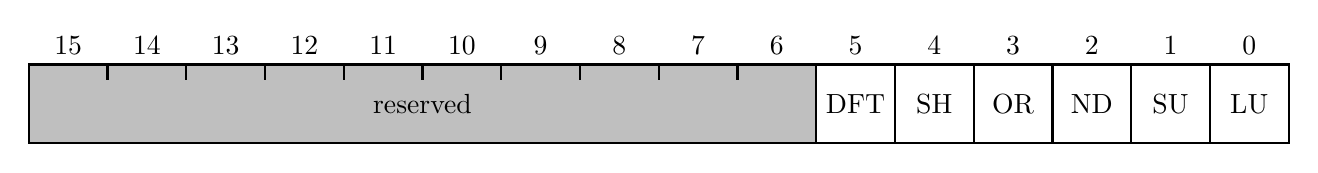
\begin{tikzpicture}
\bitrect{16}{16-\bit}
\robits{0}{10}{reserved}
\rwbits{10}{1}{DFT}
\rwbits{11}{1}{SH}
\rwbits{12}{1}{OR}
\rwbits{13}{1}{ND}
\rwbits{14}{1}{SU}
\rwbits{15}{1}{LU}
\end{tikzpicture}
\end{center}
\begin{itemize}
\item \textbf{DFT:} New DFT result available (see section~\ref{dft}).
\item \textbf{SH:} Sweep halted due to halt bit set. Sweep will be resumed once the resume command is issued.
\item \textbf{OR:} Data overrun occured (only cleared by resetting the FPGA)
\item \textbf{ND:} New data available
\item \textbf{SU:} Source unlocked
\item \textbf{LU:} LO unlocked
\end{itemize}
\subsection{Writing a register}
Writing a register requires the transfer of two words: First the control word selecting the destination address and a second word containing the new register value:
\begin{center}
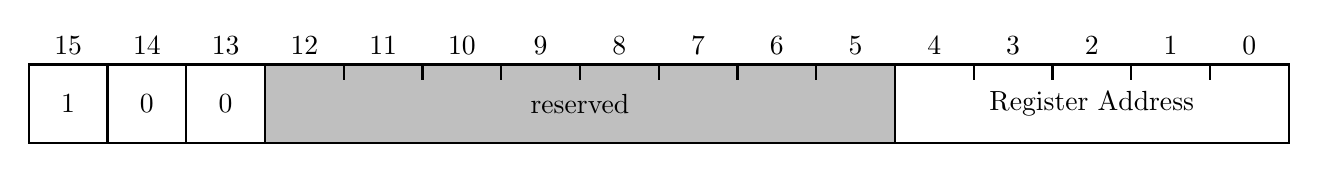
\begin{tikzpicture}
\bitrect{16}{16-\bit}
\rwbits{0}{1}{1}
\rwbits{1}{1}{0}
\rwbits{2}{1}{0}
\robits{3}{8}{reserved}
\rwbits{11}{5}{Register Address}
\end{tikzpicture}
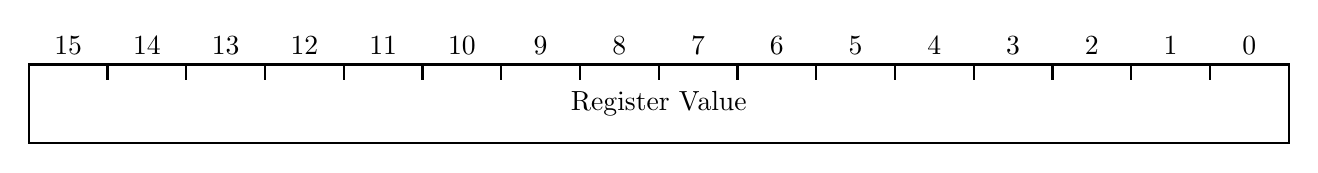
\begin{tikzpicture}
\bitrect{16}{16-\bit}
\rwbits{0}{16}{Register Value}
\end{tikzpicture}
\end{center}
\subsection{Writing SweepConfig}
Initiate the sweep config transfer by sending the command word:
\begin{center}
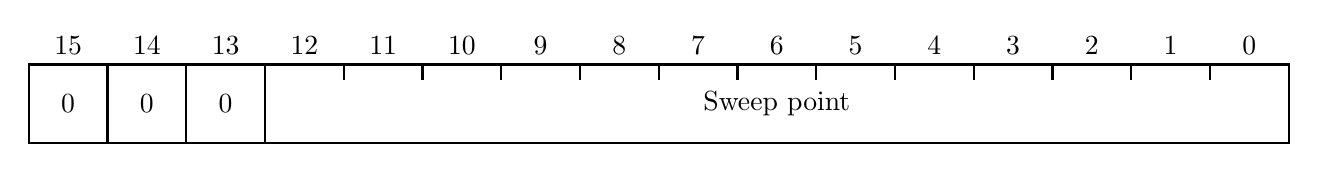
\begin{tikzpicture}
\bitrect{16}{16-\bit}
\rwbits{0}{1}{0}
\rwbits{1}{1}{0}
\rwbits{2}{1}{0}
\rwbits{3}{13}{Sweep point}
\end{tikzpicture}
\end{center}
The maximum number of points per sweep is 4501, thus the highest valid value for "Sweep point" is 4500. After the control word, send the six words of the sweep config (see section~\ref{sweepconfig}) while keeping NSS low. The sweep config is transmitted MSB first.

\subsection{Reading a sampling result}
Whenever the ND bit in the interrupt status register is set, new sampling data is available and can be read via SPI. It has to be read before the next sampling data arrives otherwise the old data will be overwritten.

Initiate the reading of sampling data by sending the command word:
\begin{center}
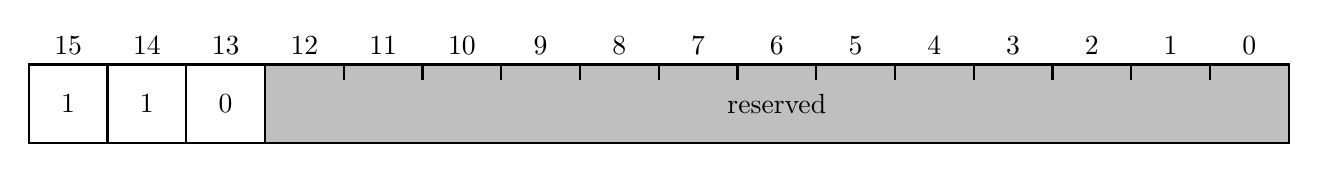
\begin{tikzpicture}
\bitrect{16}{16-\bit}
\rwbits{0}{1}{1}
\rwbits{1}{1}{1}
\rwbits{2}{1}{0}
\robits{3}{13}{reserved}
\end{tikzpicture}
\end{center}
Afterwards, read up to 19 words before setting NSS high. These 19 words will contain the sampling result (see section~\ref{result}), transmitted with the least significant word first.

\subsection{Resuming a halted sweep}
When the halt bit is set in the SweepConfig, the FPGA will configure the Source and LO as requested but will not start the settling timer (and subsequently the sampling process) until this resume command is issued. The halted sweep is indicated by the sweep halted bit in the status register.
\begin{center}
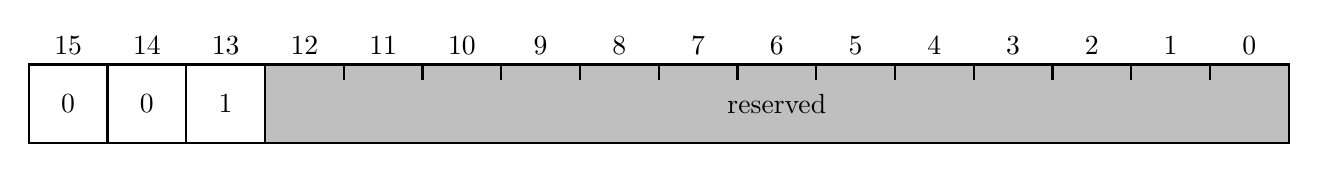
\begin{tikzpicture}
\bitrect{16}{16-\bit}
\rwbits{0}{1}{0}
\rwbits{1}{1}{0}
\rwbits{2}{1}{1}
\robits{3}{13}{reserved}
\end{tikzpicture}
\end{center}

\subsection{Reading ADC limits}
The FPGA keeps track of the highest and lowest sample of each ADC to detect saturation and verify signal levels.

Initiate the reading of ADC limit data by sending the command word:
\begin{center}
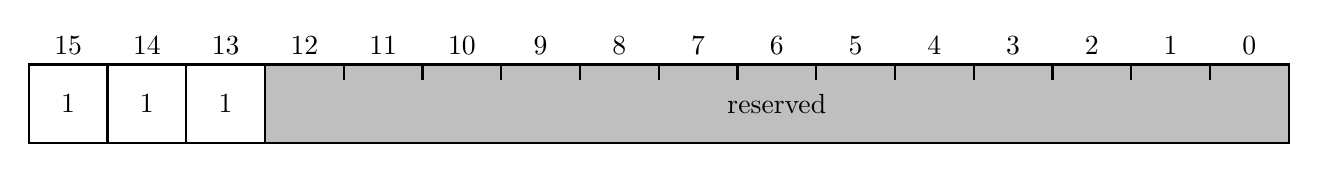
\begin{tikzpicture}
\bitrect{16}{16-\bit}
\rwbits{0}{1}{1}
\rwbits{1}{1}{1}
\rwbits{2}{1}{1}
\robits{3}{13}{reserved}
\end{tikzpicture}
\end{center}
Afterwards, read 6 words before setting NSS high. These 6 words will contain the sampling result:

\begin{center}
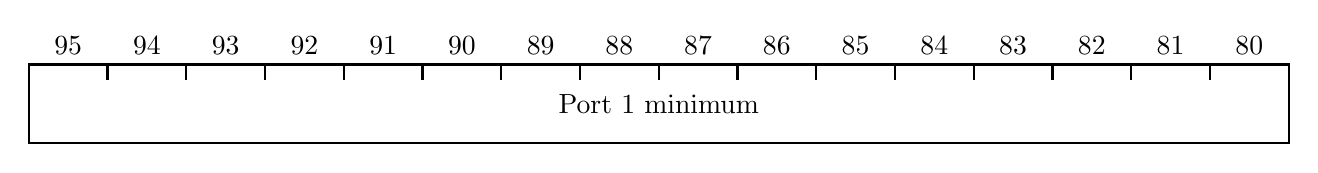
\begin{tikzpicture}
\bitrect{16}{96-\bit}
\rwbits{0}{16}{Port 1 minimum}
\end{tikzpicture}
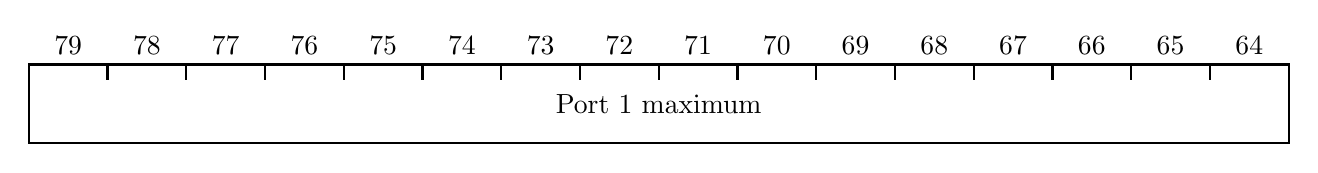
\begin{tikzpicture}
\bitrect{16}{80-\bit}
\rwbits{0}{16}{Port 1 maximum}
\end{tikzpicture}
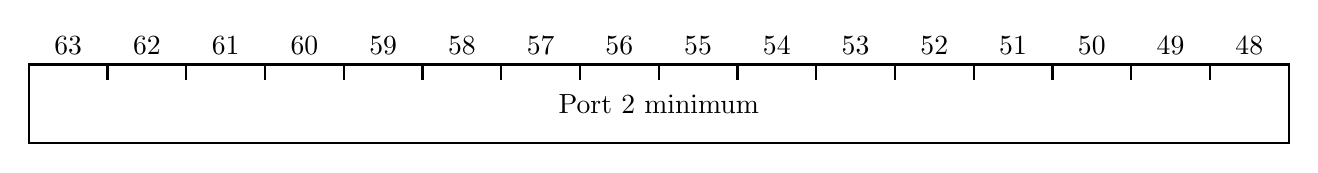
\begin{tikzpicture}
\bitrect{16}{64-\bit}
\rwbits{0}{16}{Port 2 minimum}
\end{tikzpicture}
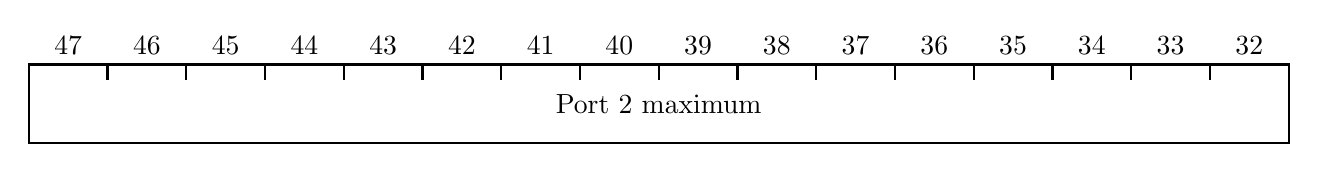
\begin{tikzpicture}
\bitrect{16}{48-\bit}
\rwbits{0}{16}{Port 2 maximum}
\end{tikzpicture}
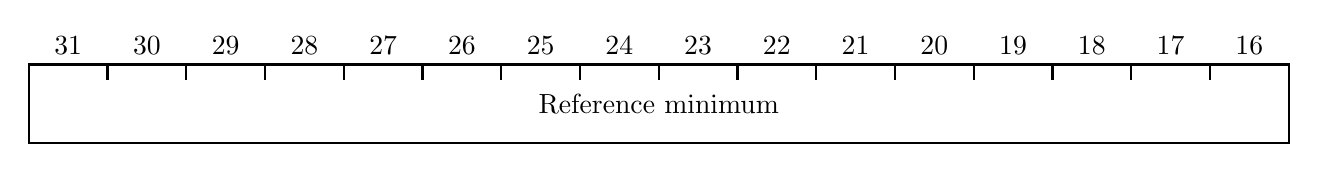
\begin{tikzpicture}
\bitrect{16}{32-\bit}
\rwbits{0}{16}{Reference minimum}
\end{tikzpicture}
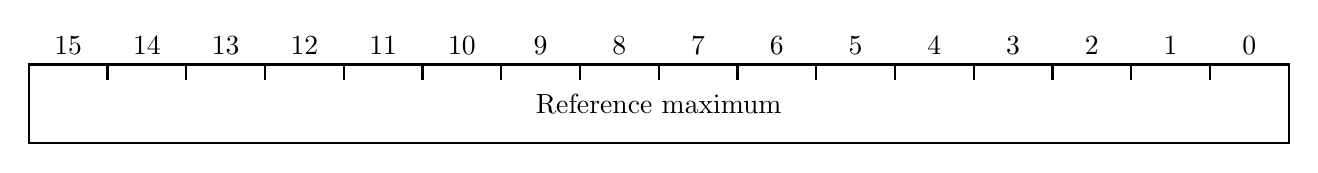
\begin{tikzpicture}
\bitrect{16}{16-\bit}
\rwbits{0}{16}{Reference maximum}
\end{tikzpicture}
\end{center}

\subsection{Resetting the ADC limit}
Issuing this command result in all minimum values set to 32767 and all maximum values set to -32768.
\begin{center}
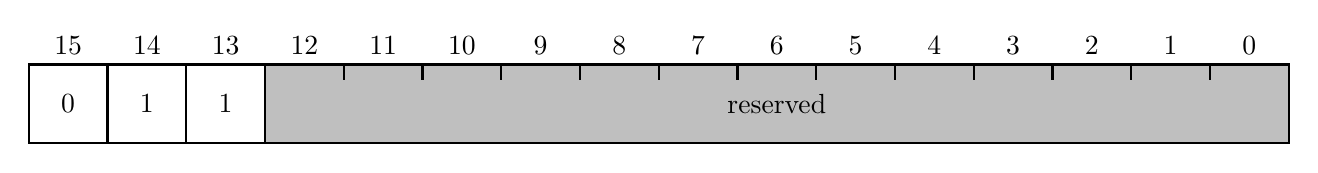
\begin{tikzpicture}
\bitrect{16}{16-\bit}
\rwbits{0}{1}{0}
\rwbits{1}{1}{1}
\rwbits{2}{1}{1}
\robits{3}{13}{reserved}
\end{tikzpicture}
\end{center}

\subsection{Reading the DFT result}
Initiate the reading of the DFT result (see section~\ref{dft}) by sending the command word:
\begin{center}
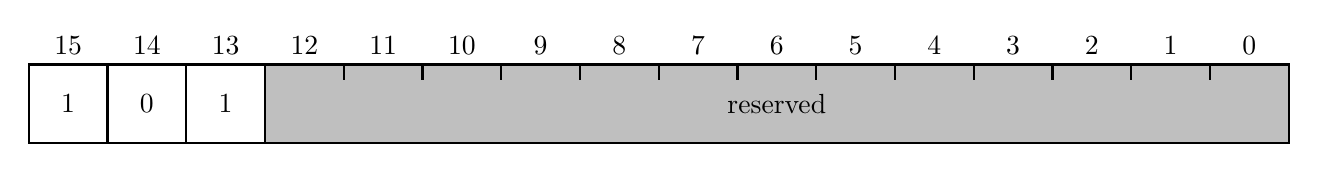
\begin{tikzpicture}
\bitrect{16}{16-\bit}
\rwbits{0}{1}{1}
\rwbits{1}{1}{0}
\rwbits{2}{1}{1}
\robits{3}{13}{reserved}
\end{tikzpicture}
\end{center}
Afterwards, read 12 words before setting NSS high. These 12 words will contain the first bin of the DFT, the least significant word is transmitted first:
\begin{center}
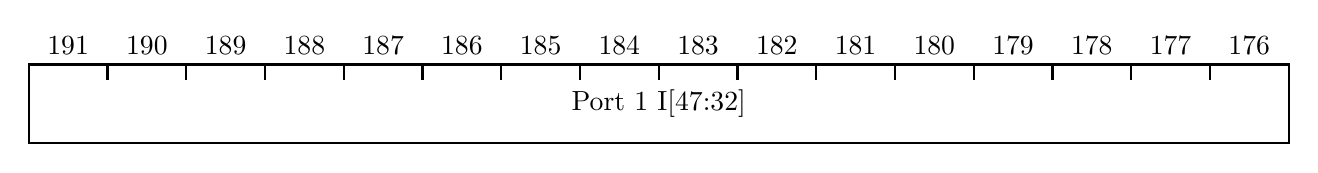
\begin{tikzpicture}
\bitrect{16}{192-\bit}
\rwbits{0}{16}{Port 1 I[47:32]}
\end{tikzpicture}
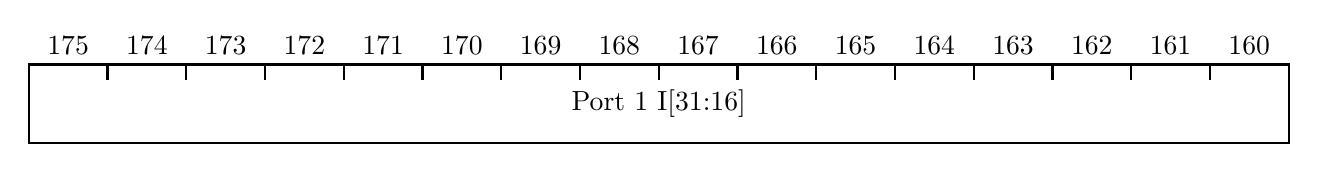
\begin{tikzpicture}
\bitrect{16}{176-\bit}
\rwbits{0}{16}{Port 1 I[31:16]}
\end{tikzpicture}
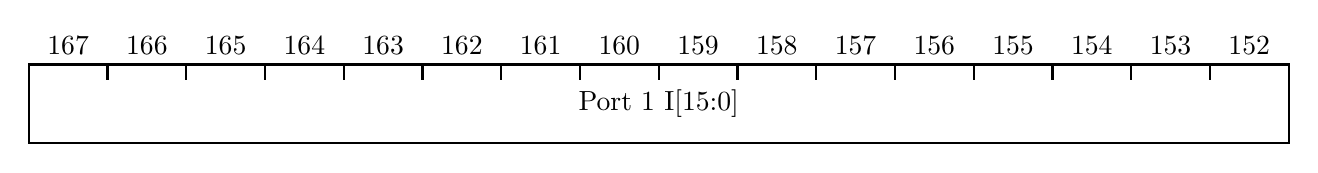
\begin{tikzpicture}
\bitrect{16}{168-\bit}
\rwbits{0}{16}{Port 1 I[15:0]}
\end{tikzpicture}
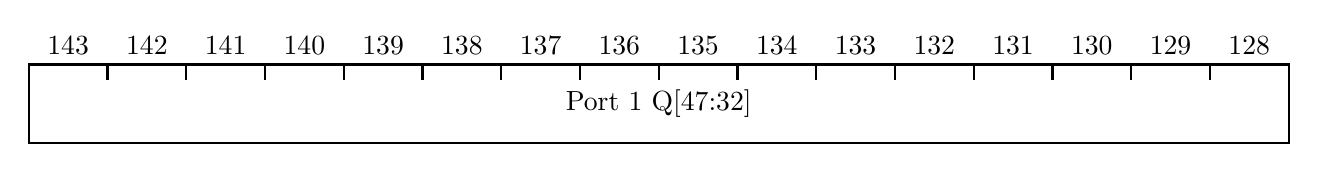
\begin{tikzpicture}
\bitrect{16}{144-\bit}
\rwbits{0}{16}{Port 1 Q[47:32]}
\end{tikzpicture}
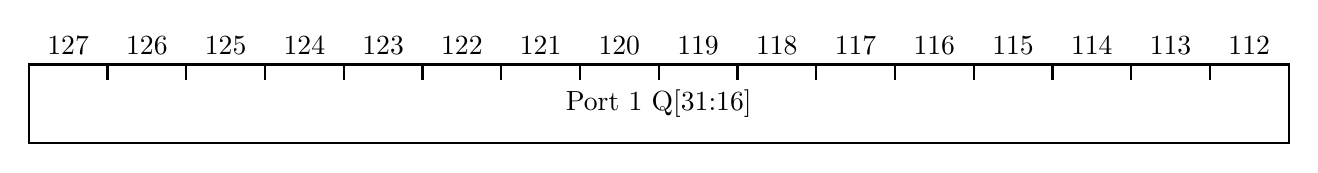
\begin{tikzpicture}
\bitrect{16}{128-\bit}
\rwbits{0}{16}{Port 1 Q[31:16]}
\end{tikzpicture}
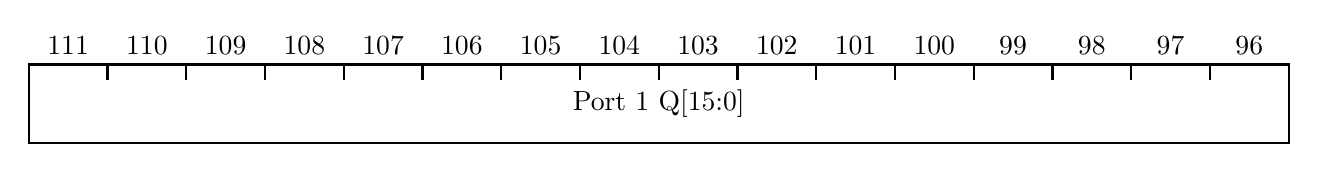
\begin{tikzpicture}
\bitrect{16}{112-\bit}
\rwbits{0}{16}{Port 1 Q[15:0]}
\end{tikzpicture}
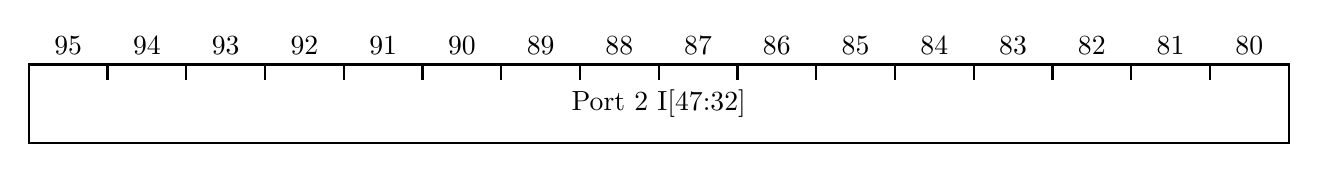
\begin{tikzpicture}
\bitrect{16}{96-\bit}
\rwbits{0}{16}{Port 2 I[47:32]}
\end{tikzpicture}
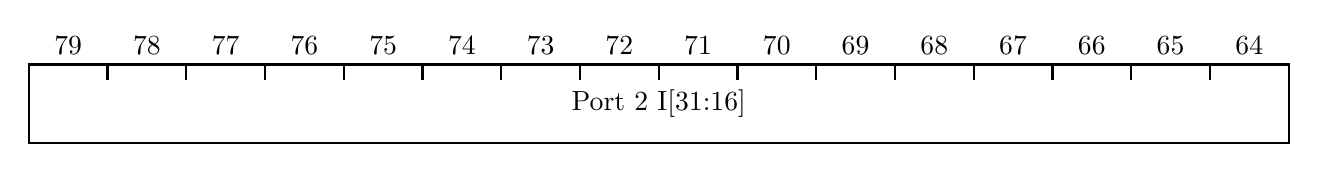
\begin{tikzpicture}
\bitrect{16}{80-\bit}
\rwbits{0}{16}{Port 2 I[31:16]}
\end{tikzpicture}
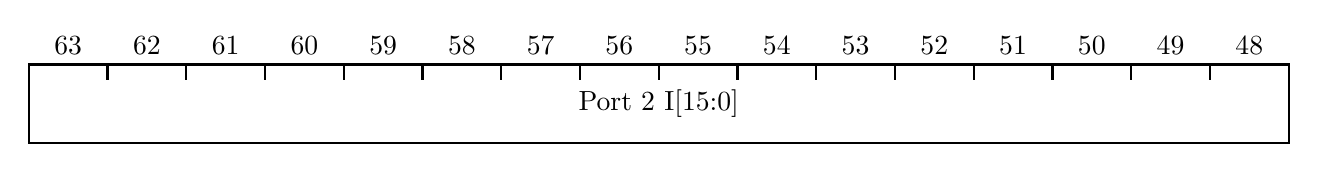
\begin{tikzpicture}
\bitrect{16}{64-\bit}
\rwbits{0}{16}{Port 2 I[15:0]}
\end{tikzpicture}
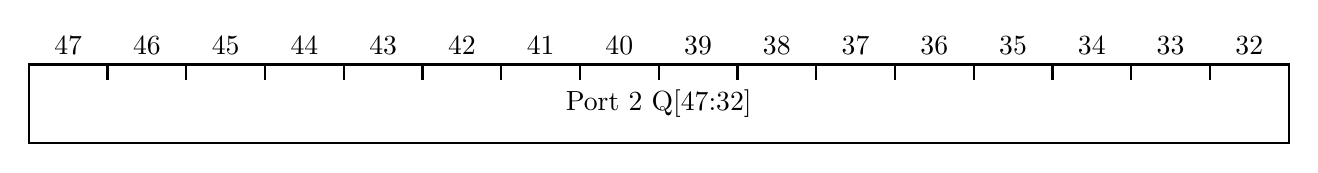
\begin{tikzpicture}
\bitrect{16}{48-\bit}
\rwbits{0}{16}{Port 2 Q[47:32]}
\end{tikzpicture}
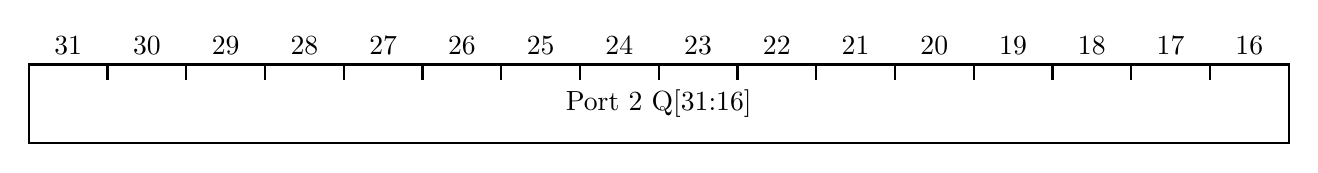
\begin{tikzpicture}
\bitrect{16}{32-\bit}
\rwbits{0}{16}{Port 2 Q[31:16]}
\end{tikzpicture}
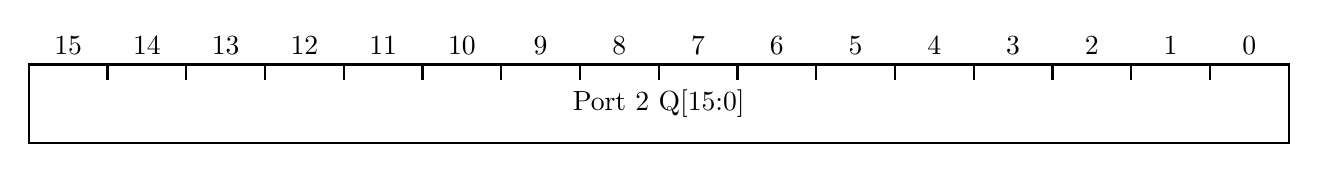
\begin{tikzpicture}
\bitrect{16}{16-\bit}
\rwbits{0}{16}{Port 2 Q[15:0]}
\end{tikzpicture}
\end{center}
Repeating this procedure will return the next DFT bin. For each bin, the CS pin has to be toggled and the command word needs to be sent again (each DFT bin requires a new SPI transaction). The DFT interrupt is reset once all bins have been read. Alternatively, toggling the DFT off and on (by disabling and enabling its interrupt) will also reset the interrupt flag.

\section{Registers}
\subsection{Interrupt Mask Register: 0x00}
\begin{center}
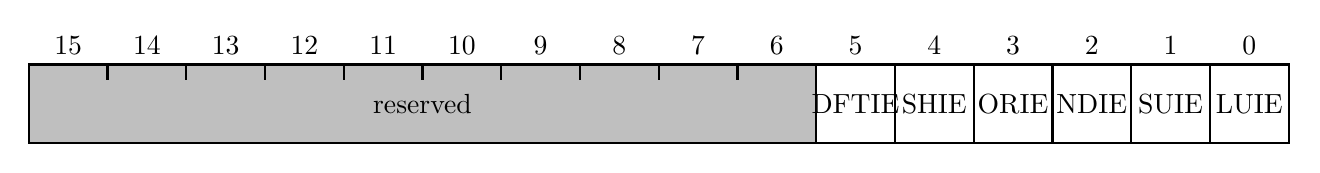
\begin{tikzpicture}
\bitrect{16}{16-\bit}
\robits{0}{10}{reserved}
\rwbits{10}{1}{DFTIE}
\rwbits{11}{1}{SHIE}
\rwbits{12}{1}{ORIE}
\rwbits{13}{1}{NDIE}
\rwbits{14}{1}{SUIE}
\rwbits{15}{1}{LUIE}
\end{tikzpicture}
\end{center}
\begin{itemize}
\item \textbf{DFTIE:} DFT interrupt enable. This bit also enables the DFT (see section~\ref{dft}).
\item \textbf{SHIE:} Sweep halted interrupt enable
\item \textbf{ORIE:} Data overrun interrupt enable 
\item \textbf{NDIE:} New data interrupt enable
\item \textbf{SUIE:} Source unlocked interrupt enable
\item \textbf{LUIE:} LO unlocked interrupt enable 
\end{itemize}

\subsection{Sweep Points Register: 0x01}
\begin{center}
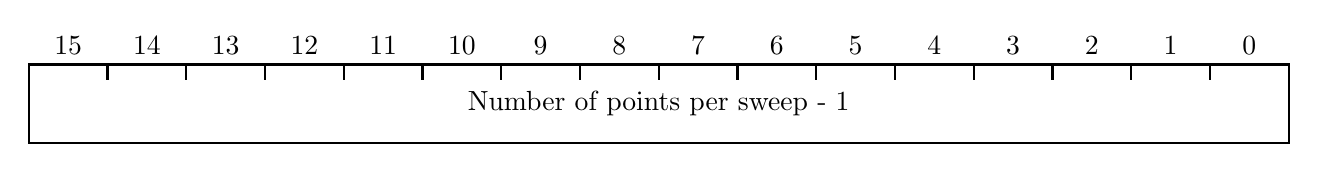
\begin{tikzpicture}
\bitrect{16}{16-\bit}
\rwbits{0}{16}{Number of points per sweep - 1}
\end{tikzpicture}
\end{center}
The register contains the number of points per sweep negative one, e.g. set to 11b if the sweep contains four points.

\subsection{Samples Per Point Register: 0x02}
\label{reg:spp}
\begin{center}
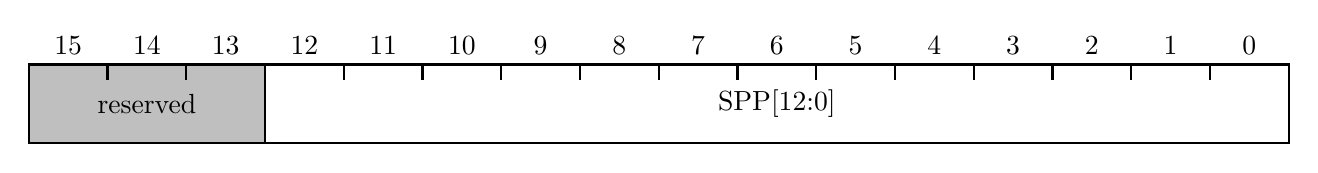
\begin{tikzpicture}
\bitrect{16}{16-\bit}
\robits{0}{3}{reserved}
\rwbits{3}{13}{SPP[12:0]}
\end{tikzpicture}
\end{center}
\begin{itemize}
\item \textbf{SPP[12:0]:} The register contains the number of samples per point in increments of 16 samples (e.g. SPP=0b0000001000=0x08 uses 128 samples per point). The value of this register is only used if SweepConfig[92:90] is set to 000. Otherwise it is overwritten for the sweep point with one of seven preselected values.
\end{itemize}

\subsection{System Control Register: 0x03}
\begin{center}
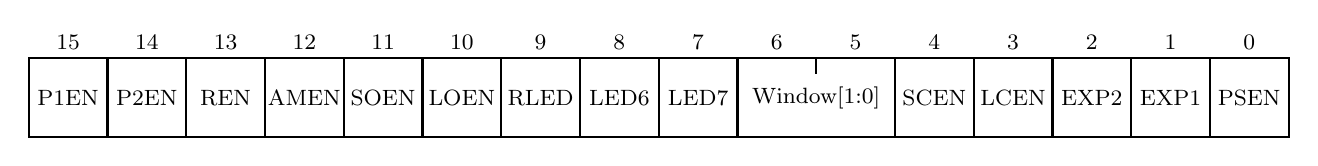
\begin{tikzpicture}
\footnotesize
\bitrect{16}{16-\bit}
\rwbits{0}{1}{P1EN}
\rwbits{1}{1}{P2EN}
\rwbits{2}{1}{REN}
\rwbits{3}{1}{AMEN}
\rwbits{4}{1}{SOEN}
\rwbits{5}{1}{LOEN}
\rwbits{6}{1}{RLED}
\rwbits{7}{1}{LED6}
\rwbits{8}{1}{LED7}
\rwbits{9}{2}{Window[1:0]}
\rwbits{11}{1}{SCEN}
\rwbits{12}{1}{LCEN}
\rwbits{13}{1}{EXP2}
\rwbits{14}{1}{EXP1}
\rwbits{15}{1}{PSEN}
\end{tikzpicture}
\end{center}
\begin{itemize}
\item \textbf{P1EN:} Port 1 Mixers/Amplifier enable
\item \textbf{P2EN:} Port 2 Mixers/Amplifier enable
\item \textbf{REN:} Reference Mixers/Amplifier enable
\item \textbf{AMEN:} Source amplifier enable
\item \textbf{SOEN:} Source enable
\item \textbf{LOEN:} LO enable
\item \textbf{RLED:} External frequency LED control
\item \textbf{LED6:}{User LED 6 control}
\item \textbf{LED7:}{User LED 7 control}
\item \textbf{Window[1:0]:}{Type of window to be used in calculation of real/imag of the sampling result}
\begin{center}
\begin{tabular}{ c|c }
Setting & Window type\\
 \hline
00 & Rectangular (no window)\\
01 & Kaiser\\
10 & Hann\\
11 & Flat Top\\
\end{tabular}
\end{center}
\item \textbf{SCEN:}{Source chip enable}
\item \textbf{LCEN:}{LO chip enable}
\item \textbf{EXP1:}{Excite Port1 during sweep}
\item \textbf{EXP2:}{Excite Port2 during sweep}
\item \textbf{PSEN:}{Port switch enable}
\end{itemize}

\subsection{ADC Prescaler register: 0x04}
\label{reg:ADC}
\begin{center}
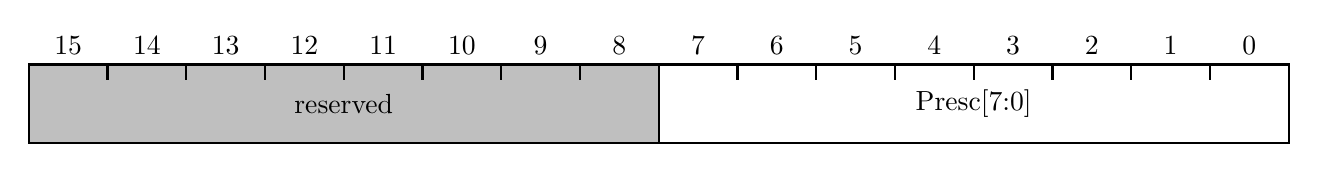
\begin{tikzpicture}
\bitrect{16}{16-\bit}
\robits{0}{8}{reserved}
\rwbits{8}{8}{Presc[7:0]}
\end{tikzpicture}
\end{center}
\begin{itemize}
\item \textbf{Presc[7:0]:} Amount of FPGA clock cycles between ADC samples.
$$ SR_{ADC} = \frac{\SI{102.4}{\mega\hertz}}{Presc} $$
The minimum value for this register is 112, which results in a samplerate of roughly \SI{914.3}{\kilo\hertz}. If Presc is set to a lower value, the data acquisition from the ADC is not done when the next sample starts and samples will be skipped.
\end{itemize}

\subsection{Phase Increment: 0x05}
\label{reg:phaseinc}
\begin{center}
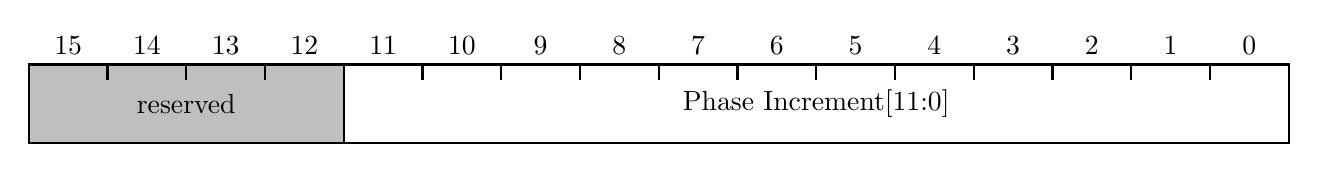
\begin{tikzpicture}
\bitrect{16}{16-\bit}
\robits{0}{4}{reserved}
\rwbits{4}{12}{Phase Increment[11:0]}
\end{tikzpicture}
\end{center}
\begin{itemize}
\item \textbf{Phase Increment[7:0]:} Phase angle between ADC samples for DFT bin calculation in $\frac{2\pi}{4096}$rad.
For a given ADC samplerate $SR_{ADC}$ and final IF frequency $f_{IF2}$ set this value to
$$ PhaseInc = \frac{4096 * f_{IF2}}{SR_{ADC}} $$
For the the default IF frequency of $f_{IF2} = \SI{250}{\kilo\hertz}$ this evaluates to 10*Presc (see ADC prescaler register).
\end{itemize}

\subsection{MAX2871 Default Values Registers: 0x08-0x0F}
See datasheet of MAX2871 for bit descriptions. Bits for the fields N, FRAC, M, VCO and DIV\_A are "don't care" as they will be overwritten by the SweepConfig setting.
\begin{center}
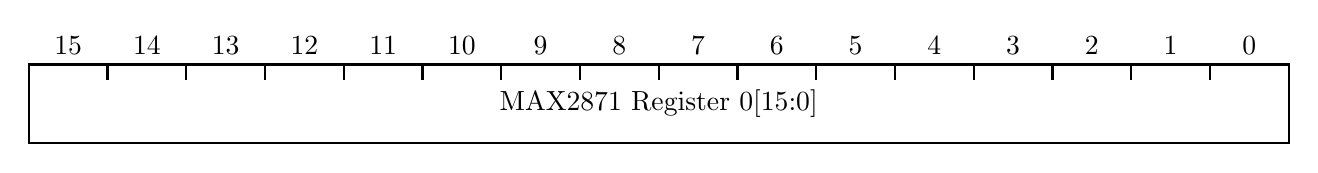
\begin{tikzpicture}
\bitrect{16}{16-\bit}
\rwbits{0}{16}{MAX2871 Register 0[15:0]}
\end{tikzpicture}
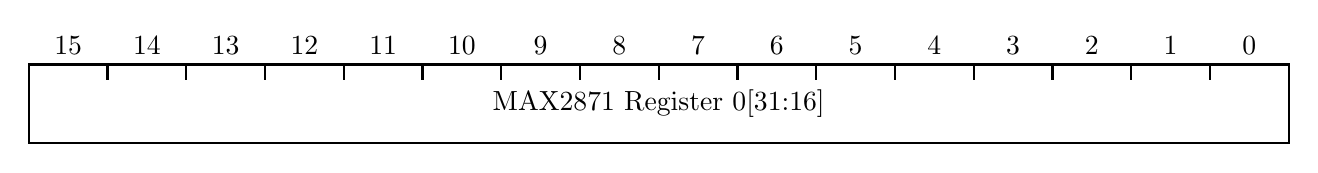
\begin{tikzpicture}
\bitrect{16}{16-\bit}
\rwbits{0}{16}{MAX2871 Register 0[31:16]}
\end{tikzpicture}
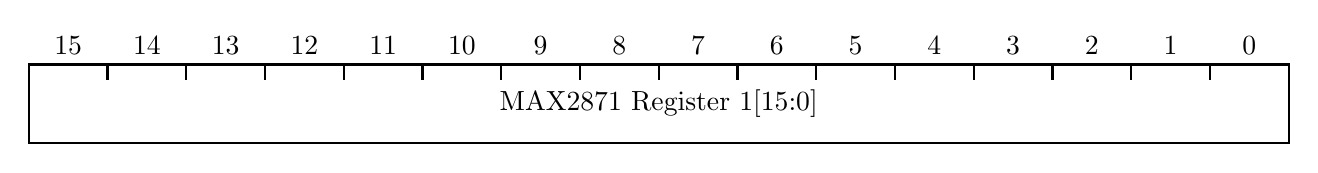
\begin{tikzpicture}
\bitrect{16}{16-\bit}
\rwbits{0}{16}{MAX2871 Register 1[15:0]}
\end{tikzpicture}
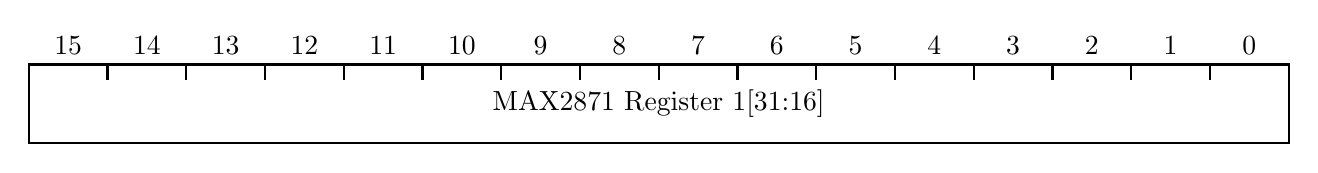
\begin{tikzpicture}
\bitrect{16}{16-\bit}
\rwbits{0}{16}{MAX2871 Register 1[31:16]}
\end{tikzpicture}
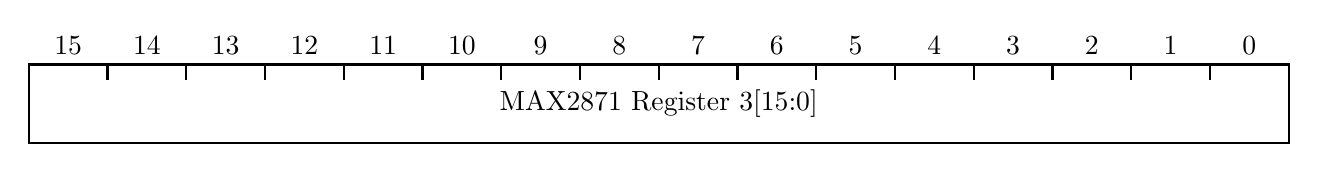
\begin{tikzpicture}
\bitrect{16}{16-\bit}
\rwbits{0}{16}{MAX2871 Register 3[15:0]}
\end{tikzpicture}
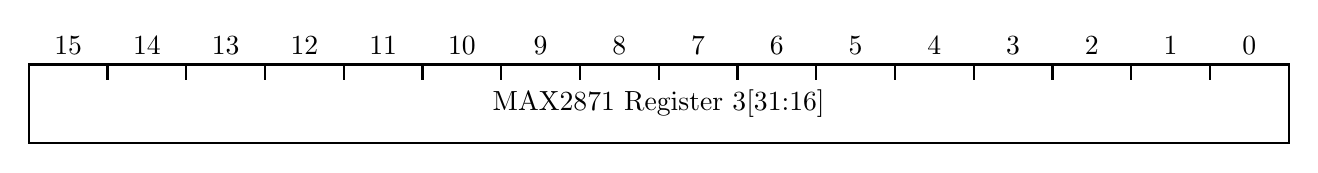
\begin{tikzpicture}
\bitrect{16}{16-\bit}
\rwbits{0}{16}{MAX2871 Register 3[31:16]}
\end{tikzpicture}
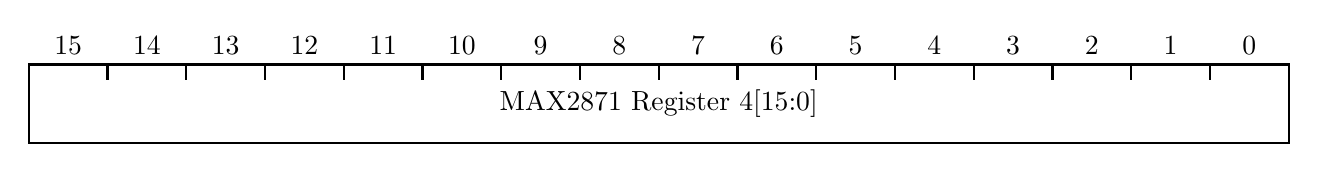
\begin{tikzpicture}
\bitrect{16}{16-\bit}
\rwbits{0}{16}{MAX2871 Register 4[15:0]}
\end{tikzpicture}
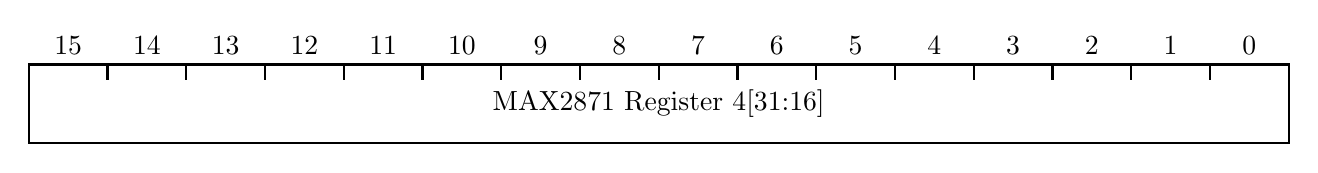
\begin{tikzpicture}
\bitrect{16}{16-\bit}
\rwbits{0}{16}{MAX2871 Register 4[31:16]}
\end{tikzpicture}
\end{center}

\subsection{DFT registers}
\label{dft}
In addition to the single bin DFT configured through the ADC prescaler and phase increment registers (see \ref{reg:ADC} and \ref{reg:phaseinc}), the FPGA also includes a multiple point DFT. This DFT only operates on the port 1 and port 2 receivers and is intended to speed up spectrum analyzer measurements. If enabled, the DFT runs in parallel to all other calculations.

The DFT has a fixed number of bins (96), but the frequencies these bins correspond to can be changed.

\subsubsection{DFT\_FIRST\_BIN: 0x12}
\begin{center}
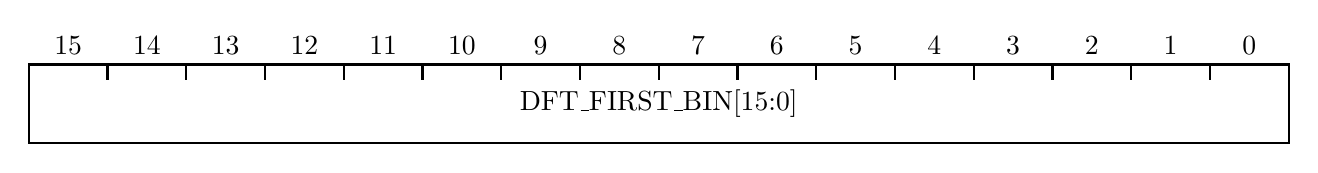
\begin{tikzpicture}
\bitrect{16}{16-\bit}
\rwbits{0}{16}{DFT\_FIRST\_BIN[15:0]}
\end{tikzpicture}
\end{center}
\begin{itemize}
\item \textbf{DFT\_FIRST\_BIN[15:0]:} This value determines the frequency corresponding to the first DFT bin.
$$ f_{firstBin} =  \frac{SR_{ADC} * DFT\_FIRST\_BIN}{2^{16}}$$
\end{itemize}

\subsubsection{DFT\_FREQ\_SPACING: 0x13}
\begin{center}
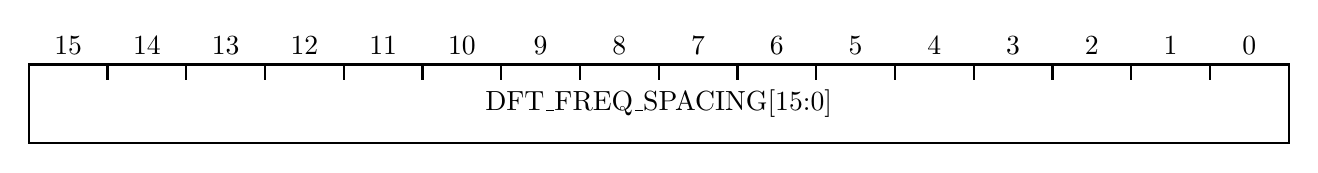
\begin{tikzpicture}
\bitrect{16}{16-\bit}
\rwbits{0}{16}{DFT\_FREQ\_SPACING[15:0]}
\end{tikzpicture}
\end{center}
\begin{itemize}
\item \textbf{DFT\_FREQ\_SPACING[15:0]:} This value determines the frequency difference between bins.
$$ \Delta f =  \frac{SR_{ADC} * DFT\_FREQ\_SPACING}{2^{24}}$$
\end{itemize}

\section{SweepConfig}
\label{sweepconfig}
The SweepConfig contains data for the source and LO1 PLL as well as the attenuator and source filter. Each point in the sweep, needs a valid SweepConfig before the sweep is started.

\begin{center}
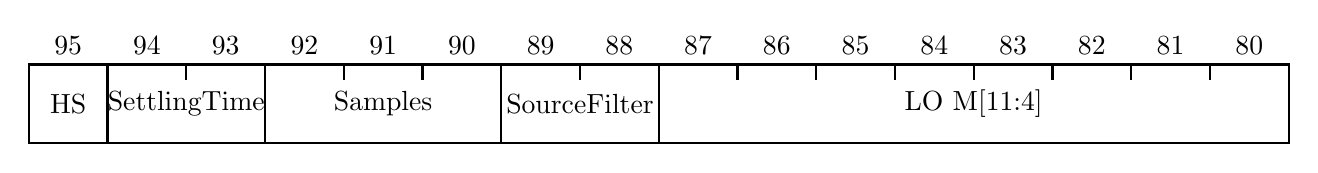
\begin{tikzpicture}
\bitrect{16}{96-\bit}
\rwbits{0}{1}{HS}
\rwbits{1}{2}{SettlingTime}
\rwbits{3}{3}{Samples}
\rwbits{6}{2}{SourceFilter}
\rwbits{8}{8}{LO M[11:4]}
\end{tikzpicture}
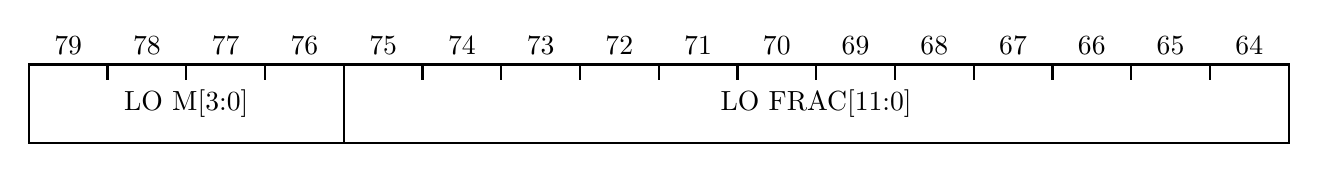
\begin{tikzpicture}
\bitrect{16}{80-\bit}
\rwbits{0}{4}{LO M[3:0]}
\rwbits{4}{12}{LO FRAC[11:0]}
\end{tikzpicture}
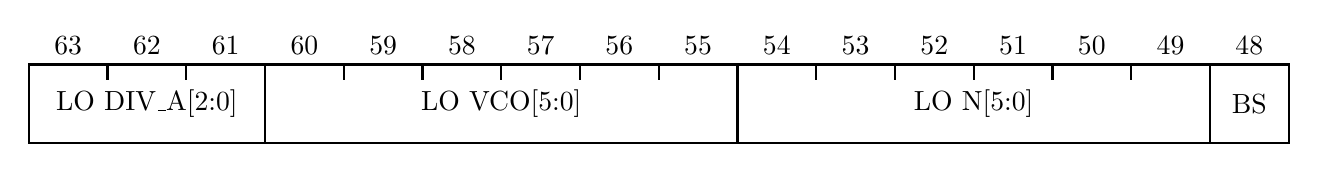
\begin{tikzpicture}
\bitrect{16}{64-\bit}
\rwbits{0}{3}{LO DIV\_A[2:0]}
\rwbits{3}{6}{LO VCO[5:0]}
\rwbits{9}{6}{LO N[5:0]}
\rwbits{15}{1}{BS}
\end{tikzpicture}
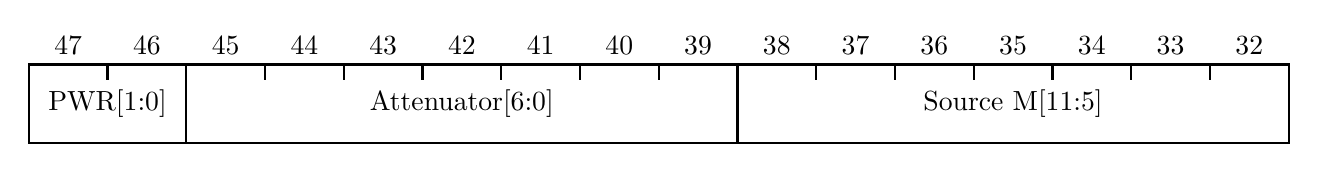
\begin{tikzpicture}
\bitrect{16}{48-\bit}
\rwbits{0}{2}{PWR[1:0]}
\rwbits{2}{7}{Attenuator[6:0]}
\rwbits{9}{7}{Source M[11:5]}
\end{tikzpicture}
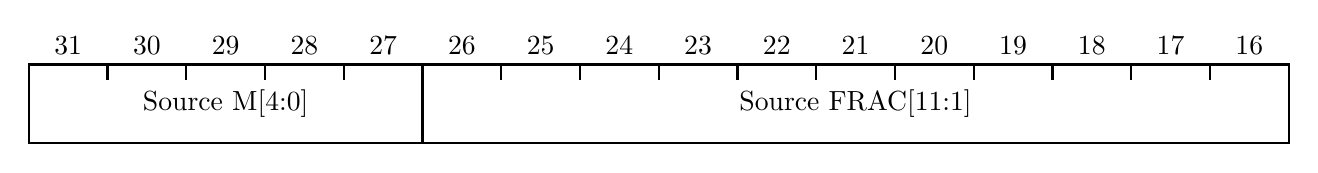
\begin{tikzpicture}
\bitrect{16}{32-\bit}
\rwbits{0}{5}{Source M[4:0]}
\rwbits{5}{11}{Source FRAC[11:1]}
\end{tikzpicture}
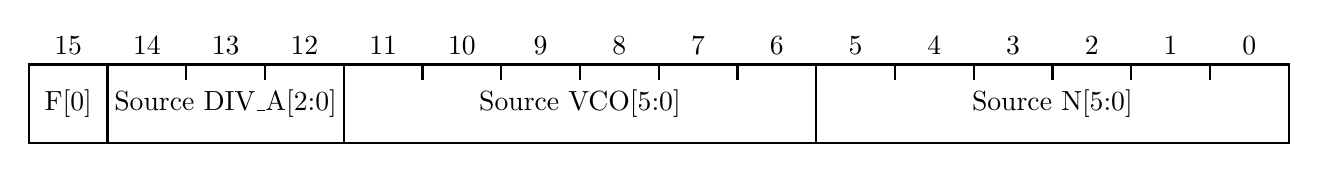
\begin{tikzpicture}
\bitrect{16}{16-\bit}
\rwbits{0}{1}{F[0]}
\rwbits{1}{3}{Source DIV\_A[2:0]}
\rwbits{4}{6}{Source VCO[5:0]}
\rwbits{10}{6}{Source N[5:0]}
\end{tikzpicture}
\end{center}
\begin{itemize}
\item \textbf{HS: Halt sweep.} If set, settling and sampling of this sweep point will be postponed until the sweep resume command is issued.
\item \textbf{SettlingTime:} Amount of time between locking of PLLs and beginning of ADC sampling
\begin{center}
\begin{tabular}{ c|c }
Setting & Time\\
 \hline
00 & \SI{20}{\micro\second}\\
01 & \SI{60}{\micro\second}\\
10 & \SI{180}{\micro\second}\\
11 & \SI{540}{\micro\second}\\
\end{tabular}
\end{center}
\item \textbf{Samples:} Number of ADC samples to take
\begin{center}
\begin{tabular}{ c|c|c }
Setting & Samples & Equivalent IF bandwidth\\
 \hline
000 & Defined by SPP register & \SI{914}{\kilo\hertz}/SPP\\
001 & 96 & \SI{10}{\kilo\hertz}\\
010 & 304 & \SI{3}{\kilo\hertz}\\
011 & 912 & \SI{1}{\kilo\hertz}\\
100 & 3040 & \SI{300}{\hertz}\\
101 & 9136 & \SI{100}{\hertz}\\
110 & 30464 & \SI{30}{\hertz}\\
111 & 91392 & \SI{10}{\hertz}\\
\end{tabular}
\end{center}
\item \textbf{SourceFilter:} Low pass filter selection for source signal
\begin{center}
\begin{tabular}{ c|c }
Setting & Selected Band\\
 \hline
00 & \SIrange{0}{900}{\mega\hertz}\\
01 & \SIrange{900}{1800}{\mega\hertz}\\
10 & \SIrange{1800}{3500}{\mega\hertz}\\
11 & \SIrange{3500}{6000}{\mega\hertz}\\
\end{tabular}
\end{center}
\item \textbf{BS: Band select.} Set to 0 for highband, set to 1 for lowband.
\item \textbf{PWR:} Power setting of source PLL. Will be written to register 4, bits [4:3] of the source PLL, controlling the output power of output A.
\begin{center}
\begin{tabular}{ c|c }
Setting & Selected Power\\
 \hline
00 & \SI{-4}{\dBm}\\
01 & \SI{-1}{\dBm}\\
10 & \SI{2}{\dBm}\\
11 & \SI{5}{\dBm}\\
\end{tabular}
\end{center}
\item \textbf{Attenuator:} Attenuation of source signal in \SI{0.25}{\decibel}.
\end{itemize}

\section{Sampling Result}
\label{result}
Each point in the sweep generates two sampling results. The first one contains the measurement when the source was routed to Port 1, the second sampling result was taken when the source was routed to Port 2. 
\begin{center}
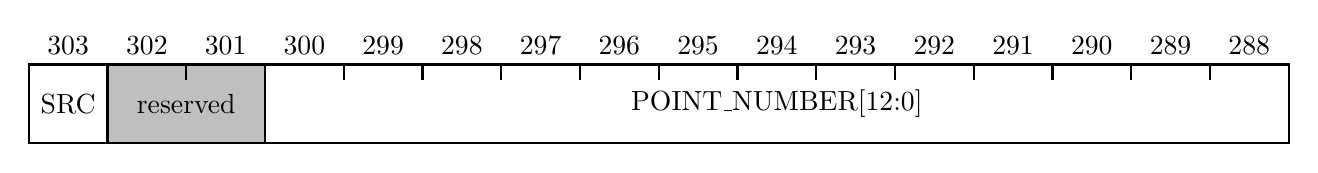
\begin{tikzpicture}
\bitrect{16}{304-\bit}
\rwbits{0}{1}{SRC}
\robits{1}{2}{reserved}
\rwbits{3}{13}{POINT\_NUMBER[12:0]}
\end{tikzpicture}
\begin{tikzpicture}
\bitrect{16}{288-\bit}
\rwbits{0}{16}{Port 1 I[47:32]}
\end{tikzpicture}
\begin{tikzpicture}
\bitrect{16}{272-\bit}
\rwbits{0}{16}{Port 1 I[31:16]}
\end{tikzpicture}
\begin{tikzpicture}
\bitrect{16}{256-\bit}
\rwbits{0}{16}{Port 1 I[15:0]}
\end{tikzpicture}

\begin{tikzpicture}
\bitrect{16}{240-\bit}
\rwbits{0}{16}{Port 1 Q[47:32]}
\end{tikzpicture}
\begin{tikzpicture}
\bitrect{16}{224-\bit}
\rwbits{0}{16}{Port 1 Q[31:16]}
\end{tikzpicture}
\begin{tikzpicture}
\bitrect{16}{208-\bit}
\rwbits{0}{16}{Port 1 Q[15:0]}
\end{tikzpicture}

\begin{tikzpicture}
\bitrect{16}{192-\bit}
\rwbits{0}{16}{Port 2 I[47:32]}
\end{tikzpicture}
\begin{tikzpicture}
\bitrect{16}{176-\bit}
\rwbits{0}{16}{Port 2 I[31:16]}
\end{tikzpicture}
\begin{tikzpicture}
\bitrect{16}{160-\bit}
\rwbits{0}{16}{Port 2 I[15:0]}
\end{tikzpicture}

\begin{tikzpicture}
\bitrect{16}{144-\bit}
\rwbits{0}{16}{Port 2 Q[47:32]}
\end{tikzpicture}
\begin{tikzpicture}
\bitrect{16}{128-\bit}
\rwbits{0}{16}{Port 2 Q[31:16]}
\end{tikzpicture}
\begin{tikzpicture}
\bitrect{16}{112-\bit}
\rwbits{0}{16}{Port 2 Q[15:0]}
\end{tikzpicture}

\begin{tikzpicture}
\bitrect{16}{96-\bit}
\rwbits{0}{16}{Reference Signal I[47:32]}
\end{tikzpicture}
\begin{tikzpicture}
\bitrect{16}{80-\bit}
\rwbits{0}{16}{Reference Signal I[31:16]}
\end{tikzpicture}
\begin{tikzpicture}
\bitrect{16}{64-\bit}
\rwbits{0}{16}{Reference Signal I[15:0]}
\end{tikzpicture}

\begin{tikzpicture}
\bitrect{16}{48-\bit}
\rwbits{0}{16}{Reference Signal Q[47:32]}
\end{tikzpicture}
\begin{tikzpicture}
\bitrect{16}{32-\bit}
\rwbits{0}{16}{Reference Signal Q[31:16]}
\end{tikzpicture}
\begin{tikzpicture}
\bitrect{16}{16-\bit}
\rwbits{0}{16}{Reference Signal Q[15:0]}
\end{tikzpicture}
\end{center}

\end{document}